\documentclass[11pt]{article} 
\usepackage{calc}
\usepackage{lettrine}
\usepackage[margin={1in,1in}]{geometry} 
\usepackage[hwkhandout]{hwk}
\usepackage[pdftitle={Chain Rule},colorlinks=true,urlcolor=blue]{hyperref}
\usepackage{graphicx}
\usepackage{wrapfig}

\renewcommand{\theclass}{\textsc{math}1300: calculus I}
\renewcommand{\theauthor}{Tyson Gern}
\renewcommand{\theassignment}{Chain Rule Worksheet}
\renewcommand{\dateinfo}{section 3.4}
\renewcommand{\abstractname}{(The Telegraph)}

\newcommand{\ds}{\displaystyle}

\begin{document}
\drawtitle
\begin{enumerate}
\item Let $h(x)=e^{2x^4-3x^3+9}$.
  \begin{enumerate}
  \item Find $f(x)$ and $g(x)$ so that $h(x)=f(g(x))$.
    \vfill
  \item Find $f'(x)$ and $g'(x)$.
    \vfill
  \item Find $h'(x)$.
    \vfill
  \end{enumerate}

\item Let $h(x)=\sqrt[3]{4^x-x^4}$
  \begin{enumerate}
  \item Find $f(x)$ and $g(x)$ so that $h(x)=f(g(x))$.
    \vfill
  \item Find $f'(x)$ and $g'(x)$.
    \vfill
  \item Find $h'(x)$.
    \vfill
  \end{enumerate}
  
\newpage

\item Let $a$ and $b$ be constants. Find the following derivatives.
  \begin{enumerate}
  \item $\ds h(x)=\left(\sqrt{\left(ax^{-1}-3x^9\right)^3}\right)^{b}$
    (\textsc{hint}: simplify algebraically \textit{first})
    \vfill
  \item $\ds h(x)=\left(4^{3x}-7\cdot 4^{2x}+b\cdot
      4^x+9\right)\cdot\sqrt{\dfrac{3}{x^2-2}}$
    \vfill
  \end{enumerate}

\newpage

\item For what intervals is $f(x) = xe^{-x}$ concave down?

\newpage

\item \textit{This question is from the book, but I thought that it
    would be good to do in class due to the recent study in physics
    concerning the speed of light (See attached article).}

The theory of relativity predicts that an object whose mass is $m_0$
when it is at rest will appear heavier when moving at speeds near the
speed of light.  When the object is moving at speed $v$ its mass $m$
is given by
\begin{equation}\tag{1}\label{light}
m = \frac{m_0}{\sqrt{1-\left(\frac{v^2}{c^2}\right)}},
\end{equation}
where $c$ is the speed of light.

\begin{enumerate}
\item Find $\dfrac{dm}{dv}$.
\vfill
\item In terms of physics, what does $\dfrac{dm}{dv}$ tell you?
\vfill

\newpage


\item The attached article describes a recent study in physics about
  the speed of light.  The findings of the study were eventually found
  to be false.  If these findings were found to be correct, how do
  would this affect equation~(\ref{light})?

  (\textsc{hint}: What happens to $m$ as $v$ approaches $c$?)

  \vspace{3.9in}
\end{enumerate}

\end{enumerate}

\hrule

\section*{Scientists did not break speed of light - it was a faulty wire}

\begin{abstract}
  \noindent Physicists who shocked the scientific world by claiming to
  have shown particles could move faster than the speed of light have
  admitted it was a mistake due to a faulty wire connection.
\end{abstract}

\begin{wrapfigure}{r}{0.4\textwidth}
  \begin{center}
    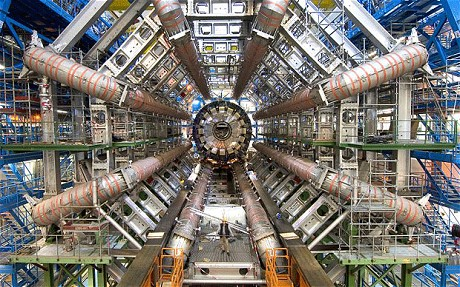
\includegraphics[width=0.38\textwidth]{cern.jpg}
  \end{center}
\end{wrapfigure}

\lettrine[lines=1]{I}{t was Albert Einstein} who proposed more than 100 years ago that
nothing could travel faster than the speed of light. 

Einstein’s theory of special relativity, proposed in 1905, states that
nothing in the universe can travel faster than the speed of light in a
vacuum.

But researchers at the CERN lab near Geneva claimed they had recorded
neutrinos, a type of tiny particle, traveling faster than the barrier
of 186,282 miles (299,792 kilometers) per second.

Now it seems Einstein's reputation has been restored after a source
close to the experiment told the US journal Science Insider that ``A
bad connection between a GPS unit and a computer may be to blame.''

Scientists at CERN claimed that neutrinos arrived 60 nanoseconds
earlier than the 2.3 milliseconds taken by light.

The report in Science Insider said the ``60 nanoseconds discrepancy
appears to come from a bad connection between a fiber optic cable that
connects to the GPS receiver used to correct the timing of the
neutrinos' flight and an electronic card in a computer.''

``After tightening the connection and then measuring the time it takes
data to travel the length of the fiber, researchers found that the
data arrive 60 nanoseconds earlier than assumed,'' it added.

``Since this time is subtracted from the overall time of flight, it
appears to explain the early arrival of the neutrinos. New data,
however, will be needed to confirm this hypothesis.''

Antonio Ereditato, spokesman for the researchers, said at the time:
``We have high confidence in our results. We have checked and
rechecked for anything that could have distorted our measurements but
we found nothing.''

Scientists across the world agreed if the results were confirmed, that
it would force a fundamental rethink of the laws of physics.

John Ellis, a theoretical physicist, said Einstein’s theory underlies
``pretty much everything in modern physics''.

The first doubt was cast on the findings In November when a team of
physicists in Italy conducting a separate study on the same beam of
neutrinos at Gran Sasso claimed their findings ``refute a superluminal
(faster than light) interpretation.''

Rather than measuring the time it took the neutrinos to travel from
CERN to Gran Sasso the second experiment, known as ICARUS, monitored
how much energy they had when they arrived.

Tomasso Dorigo, a CERN physicist, wrote on the Scientific Blogging
website that the ICARUS paper was ``very simple and definitive.''

He said it showed ``that the difference between the speed of neutrinos
and the speed of light cannot be as large as that seen by OPERA, and
is certainly smaller than that by three orders of magnitude, and
compatible with zero.''

Prof Jim Al-Khalili, the University of Surrey, who threatened to eat
his boxer shorts if the original OPERA result was proved right, said:
``Usually we see this effect when particles go faster than light
through transparent media like water, when light is considerably
slowed down.

``So these neutrinos should have been spraying out particles like
electrons and photons in a similar way if they were going superluminal
– and in the process would be losing energy.

``But they seemed to have kept the energy they started from, which
rules out faster-than-light travel.''

\vfill

\bibliographystyle{plain}
\nocite{*}
\bibliography{03.04refs}

\end{document}

%%%%%%%%%%%%%%%%%%%%%%%%%%%%%%%%%%%%%%%%%%%%%%%%%%%%%%%%%%%%%%%%%%%%%%
%%% Local Variables:
%%% mode: TeX-PDF
%%% End:
%%%%%%%%%%%%%%%%%%%%%%%%%%%%%%%%%%%%%%%%%%%%%%%%%%%%%%%%%%%%%%%%%%%%%%